\documentclass{beamer}

\usepackage{comment}
\usepackage{color}
\usepackage{listings}
\usepackage{verbatim}
\usepackage{multicol}
\usepackage{booktabs}
\definecolor{green}{RGB}{0,128,0}

\newcommand\gehcomment[1]{{{\color{orange} #1}}}
\newcommand\add[1]{{{\color{blue} #1}}}
\newcommand\remove[1]{\sout{{\color{red} #1}}}
\newcommand\codecomment[1]{{{\color{green} #1}}}
\newcommand\redcomment[1]{{{\color{red} #1}}}
\newcommand\bluecomment[1]{{{\color{blue} #1}}}
\newcommand\greencomment[1]{{{\color{green} #1}}}
\newcommand\magentacomment[1]{{{\color{magenta} #1}}}

\begin{comment}
\tiny
\scriptsize
\footnotesize
\small
\normalsize
\large
\Large
\LARGE
\huge
\Huge
\end{comment}

\begin{document}
\title{Challenge Problem}
\author{Emily Stein}
\date{\today}

%\frame{\titlepage}

%-----------------------------------------------------------------------------
\section{Location of Example}

\begin{frame}[fragile,containsverbatim]\frametitle{Location}

Location of the challenge problem:

\begin{semiverbatim}
> cd \$PFLOTRAN_DIR
> cd shortcourse/exercises/challenge_problem
> ls

kryptonite_conc.py \bluecomment{! to plot concentrations when done}
kryptonite.dat     \bluecomment{! chemistry database for you to use}
kryptonite.in      \bluecomment{! the answer - DO NOT USE THIS!!!!}
kryptonite_vf.py   \bluecomment{! to plot mineral volume fractions}
\end{semiverbatim}

\end{frame}

%-----------------------------------------------------------------------------
\section{Description of Challenge Problem}

\subsection{Kryptonite Conceptual Model}

\begin{frame}\frametitle{Description of Kryptonite Scenario}
Challenge yourself by setting up an input deck to simulate the ``\gehcomment{Kryptonite Scenario}.'' It features:
\begin{itemize}
  \item Problem domain: $2000 \times 1 \times 800$ m (x $\times$ y $\times$ z)
  \item \redcomment{Structured grid} with your choice of discretization
  \item SUBSURFACE\_FLOW MODE \redcomment{RICHARDS}
  \item \redcomment{Hydrostatic} initial conditions
  \item Regional pressure gradient (\redcomment{Dirichlet} boundary conditions)
  \item Extraction well (a \redcomment{sink})
  \item Recharge (\redcomment{Neumann} boundary condition)
  \item SUBSURFACE\_TRANSPORT
  \item Aqueous, solid, sorbed phases, radioactive decay
\end{itemize}

\end{frame}

%-----------------------------------------------------------------------------
\frame{\frametitle{2D Kryptonite Scenario Schematic}
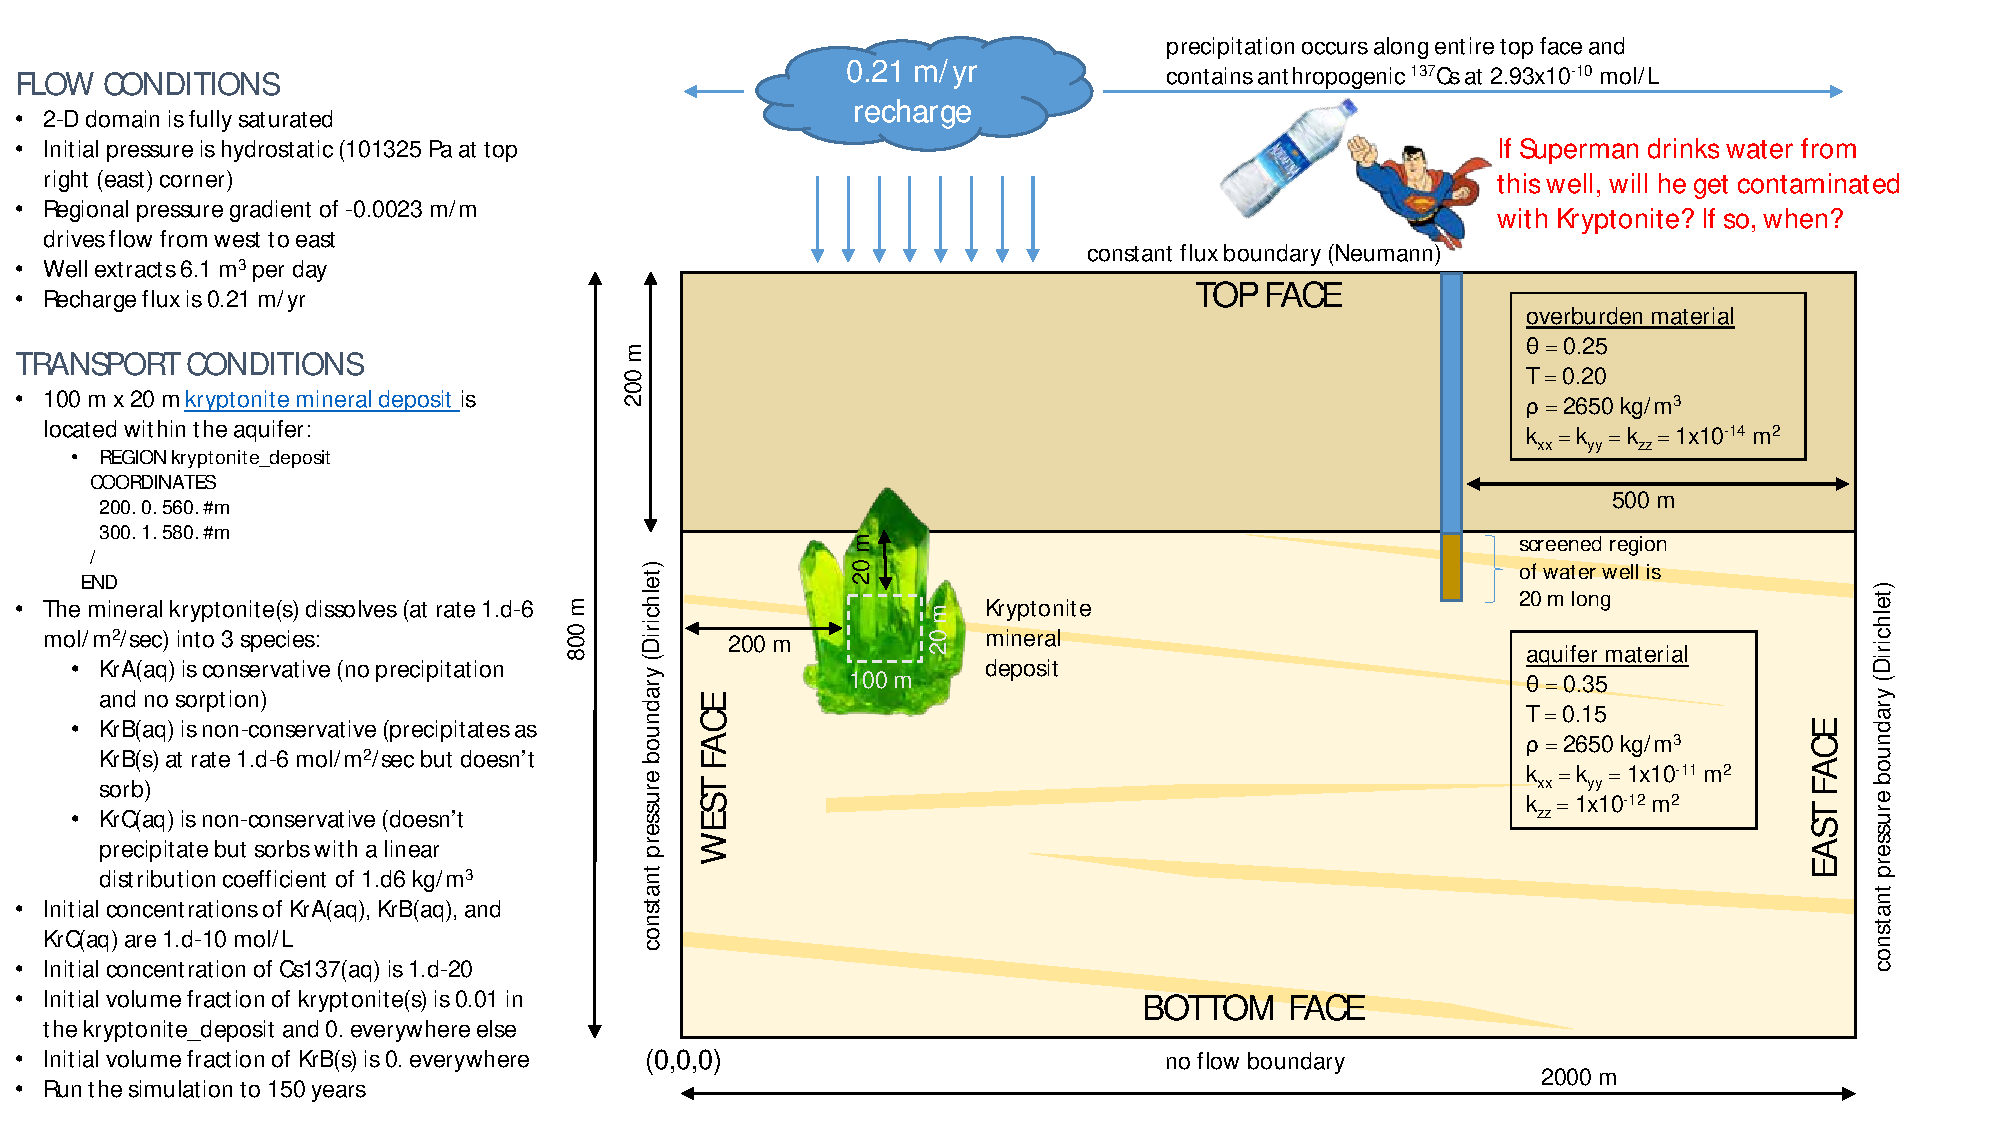
\includegraphics[width=\linewidth]{./kryptonite_schematic}
}

%-----------------------------------------------------------------------------
\section{Description of Problem}

%-----------------------------------------------------------------------------
\subsection{The Problem}

\begin{frame}[fragile]\frametitle{The Problem}
Superman drinks from a well downgradient of a kryptonite deposit. The kryptonite dissolves into three components:

\begin{itemize}
  \item At 1e-3 M, \greencomment{KrA(aq)} will make Superman weak
  \item At 1e-3 M, \greencomment{KrB(aq)} will make Superman very weak
  \item At 1e-3 M, \greencomment{KrC(aq)} will bring Superman to the brink of death
\end{itemize}

\begin{itemize}
  \item Will kryptonite contaminate the well at levels Superman should avoid? 
  \item When should Superman avoid drinking water from the well if he wants to avoid damage from \greencomment{KrA(aq)}, \greencomment{KrB(aq)}, and \greencomment{KrC(aq)}?
\end{itemize}

\end{frame}

%-----------------------------------------------------------------------------
\subsection{More Questions}

\begin{frame}[fragile]\frametitle{More Questions}
After the kryptonite deposit dissolves completely, Superman will no longer have to worry about his well water.

\begin{itemize}
  \item At what time does \greencomment{kryptonite(s)} completely dissolve?
  \item When does the concentration of \greencomment{KrA(aq)} at the well drop below 1e-3 M?
  \item Why does \greencomment{KrB(aq)} remain at 1e-3 M for a longer time?
\end{itemize}

\end{frame}

%-----------------------------------------------------------------------------
\subsection{For Mere Humans}

\begin{frame}[fragile]\frametitle{For Mere Humans}
Superman isn't affected by \greencomment{Cs137(aq)}, but humans have set an effluent limit of approximately 8.4e-14 M. Assuming water is okay to drink if the concentration of \greencomment{Cs137(aq)} $<$ 8.4e-14 M:

\begin{itemize}
  \item When is it okay for a mere human to drink water from Superman's well?
\end{itemize}

\end{frame}

%-----------------------------------------------------------------------------
\subsection{Getting Started}

\begin{frame}[fragile]\frametitle{Getting Started}
Copy 1D\_Calcite/flow\_and\_tran.in to mykryptonite.in and begin editing.
\begin{semiverbatim}
  > cp ../1D\_Calcite/flow\_and\_tran.in mykryptonite.in
  > vi mykryptonite.in \bluecomment{(or use text editor of choice)}
\end{semiverbatim}
Avoid having to debug multiple changes at once. Make one set of changes at a time and try out your simulation.
\begin{semiverbatim}
  > pflotran -input\_prefix mykryptonite
\end{semiverbatim}
Use documentation at \bluecomment{documentation.pflotran.org}
-
Put an observation point in the well and one in the kryptonite deposit. Copy kryptonite.py to mykryptonite.py and edit file paths and column numbers to plot concentrations.
\begin{semiverbatim}
  > cp kryptonite.py mykryptonite.py
  > vi mykryptonite.py \bluecomment{(or use text editor of choice)}
  > python mykryptonite.py
\end{semiverbatim}

\end{frame}

%-----------------------------------------------------------------------------
\subsection{If You Get Stuck}

\begin{frame}[fragile]\frametitle{If You Get Stuck}
Create a clean copy of mykryptonite.in
\begin{semiverbatim}
  > cp ../1D\_Calcite/flow\_and\_tran.in mykryptonite.in
\end{semiverbatim}
1. Grab a real characteristic curve first
\begin{itemize}\small
  \item{CHARACTERISTIC\_CURVES (copy from regional\_doublet.in)}
\end{itemize}
2. Change the grid discretization and corresponding regions
\begin{itemize}\small
  \item{GRID, REGION all, REGION west, REGION east}
\end{itemize}
Make sure your input deck runs after each edit
\begin{semiverbatim}
  > pflotran -input\_prefix mykryptonite
\end{semiverbatim}
\end{frame}

\begin{frame}[fragile]\frametitle{If You Get Stuck, continued}
3. Set up the new flow problem
\begin{itemize}\small
  \item{FLOW\_CONDITION initial\_pressure, BOUNDARY\_CONDITION inlet}
  \item{FLOW\_CONDITION inlet\_flux becomes FLOW\_CONDITION recharge}
  \item{create REGION top, BOUNDARY\_CONDITION top}
  \item{create FLOW\_CONDITION extraction, REGION well, SOURCE\_SINK}
\end{itemize}
Make sure your input deck runs after each edit
\begin{semiverbatim}
  > pflotran -input\_prefix mykryptonite
\end{semiverbatim}
\end{frame}

\begin{frame}[fragile]\frametitle{If You Get Stuck, continued}
4. Set up the new chemistry problem - make sure species names match those in \greencomment{kryptonite.dat}
\begin{itemize}\small
  \item{PRIMARY\_SPECIES, MINERALS, MINERAL\_KINETICS, CONSTRAINTs}
  \item{REGION kryptonite\_deposit, TRANSPORT\_CONDITION, INITIAL\_CONDITION}
  \item{CONSTRAINT rain, TRANSPORT\_CONDITION, BOUNDARY\_CONDITION top}
\end{itemize}
5. Add sorption and radioactive decay (\bluecomment{documentation.pflotran.org})
\begin{itemize}\small
  \item{SORPTION (ISOTHERM\_REACTIONS),ROCK\_DENSITY}
  \item{RADIOACTIVE\_DECAY\_REACTION}
\end{itemize}
Make sure your input deck runs after each edit
\begin{semiverbatim}
  > pflotran -input\_prefix mykryptonite
\end{semiverbatim}
\end{frame}

\begin{frame}[fragile]\frametitle{If You Get Stuck, continued}
6. Split into two strata (overburden and aquifer materials)
\begin{itemize}\small
  \item{REGION, MATERIAL\_PROPERTY, STRATA blocks for each}
\end{itemize}
7. Add observation points
\begin{itemize}\small
  \item{REGIONs, OBSERVATIONs, OUTPUT}
\end{itemize}
8. Adjust final time and time stepping
\begin{itemize}\small
  \item{TIME}
\end{itemize}
9. Add a convergence check on pressure update
\begin{itemize}\small
  \item{NEWTON\_SOLVER ITOL\_UPDATE 1.d0 END}
\end{itemize}
Make sure your input deck runs after each edit
\begin{semiverbatim}
  > pflotran -input\_prefix mykryptonite
\end{semiverbatim}
\redcomment{THAT SHOULD DO IT!} Try plotting
\begin{semiverbatim}
  > python kryptonite_conc.py
  > python kryptontite_vf.py
\end{semiverbatim}

\end{frame}
%-----------------------------------------------------------------------------
\subsection{BONUS 1}

\begin{frame}[fragile]\frametitle{Bonus \#1}
Time steps or grid cells that are too large introduce numerical dispersion.

\begin{itemize}
  \item Does decreasing MAXIMUM\_TIMESTEP\_SIZE change your answers?
  \item Does decreasing the size of grid cells change your answers?
\end{itemize}

\end{frame}

%-----------------------------------------------------------------------------
\subsection{BONUS 2}

\begin{frame}[fragile]\frametitle{Bonus \#2}
Play with increasing the recharge at the top boundary and decreasing the pressure gradient from west to east until Superman doesn't have to worry about his drinking water. 

\begin{itemize}
  \item What combinations of recharge and pressure gradient prevent kryptonite from reaching the well?
\end{itemize}

\end{frame}

%-----------------------------------------------------------------------------
\subsection{BONUS 3}

\begin{frame}[fragile]\frametitle{Bonus \#3}
Play with the model domain.

\begin{itemize}
  \item Use DXYZ instead of BOUNDS in the GRID block
  \item Add the third dimension to the domain by making the Y dimension 200 m and discretizing it
  \item Discretize a 1-m wide well that extends from x = 1499. to 1500. and y = 99. to 100.
  \item Don't forget to adjust the COORDINATES of REGION kryptonite\_deposit
  \item How does adding the third dimension affect concentrations at the well?
\end{itemize}

\end{frame}

%-----------------------------------------------------------------------------
\subsection{BONUS 4}

\begin{frame}[fragile]\frametitle{Bonus \#4}
Add an unsaturated zone to the initial condition.

\begin{itemize}
  \item Modify the HYDROSTATIC initial condition to create a 20 m thick unsaturated zone at the top of the model domain
  \item Hint: use the DATUM
  \item How long does the unsaturated zone persist? How does this initial condition affect concentrations at the well?
\end{itemize}

\end{frame}

%-----------------------------------------------------------------------------
\subsection{BONUS 5}

\begin{frame}[fragile]\frametitle{Bonus \#5}
Give the aquifer heterogeneous permeability.

\begin{itemize}
  \item Make the number of grid cells the same as in regional\_doublet/stochastic\_regional\_doublet.in
  \item Use a heterogeneous permeability field (in perm\_fields.h5) from that problem in MATERIAL\_PROPERTY aquifer
  \item (This domain will be large enough that running on 8 cores is preferable.)
  \item How does heterogeneous permeability affect the outcome at the well?
\end{itemize}

\end{frame}

%-----------------------------------------------------------------------------
\subsection{BONUS 6}

\begin{frame}[fragile]\frametitle{Bonus \#6}
Add a heat source to REGION kryptonite\_deposit. You choose the wattage.

\begin{itemize}
  \item Set the problem up in SUBSURFACE\_FLOW MODE TH
  \item Hint: See geologic\_disposal/gdsa.in for help with FLOW\_CONDITION and SOURCE\_SINK blocks
  \item You'll also need to change CHARACTERISTIC\_CURVES to SATURATION\_FUNCTIONS
  \item How does the heat source affect the flow solution? Can you see its effect in concentrations at the well?
\end{itemize}

\end{frame}

%-----------------------------------------------------------------------------
\end{document}
